pippo
\subsection{Simmetrie e leggi di conservazione}
In generale una legge fisica è simmetrica rispetto ad una trasformazione quando la forma della legge è invariante per questa trasformazione. Sia in meccanica classica che quantistica. 
\begin{itemize}
    \item In QM se l'operatore non dipende esplicitamente dal tempo allora commuta con la hamiltoniana del sistema. In generale (non sempre?) i numeri quantici conservati sono associati ad operatori che commutano con l'hamiltoniana.
    \item Le simmetrie si dividono in continue e discrete. Vediamo ad esempio la traslazione spaziale (continua)
    \begin{equation*}
        \psi(r+\delta r)=\psi(r)+\delta r \dv{\psi}{r}=\qty(1+\delta r \pdv{}{r})\psi(r)
    \end{equation*}
    L'operatore che descrive una traslazione finita è l'impulso:
    \begin{equation*}
        D=1+\frac i\hbar p\delta r\implies D=\lim_n\qty(1+\frac {ip\Delta r}{n\hbar})^n=e^{\frac i\hbar p\Delta r}
    \end{equation*}
    Chiamiamo $p$ generatore dell'operatore $D$ di traslazione spaziale. Se l'hamiltoniana è invariante per traslazioni, allora commuta con $D$ e dunque anche con $p$. Questo lo si può esprimere in tre modi equivalenti:
    \begin{enumerate}
        \item L'impulso si conserva in un sistema isolato.
        \item L'hamiltoniana è invariante per traslazioni spaziali.
        \item L'operatore impulso commuta con l'hamiltoniana.
    \end{enumerate}
    \item A simmetrie continue associamo numeri quantici additivi, a simmetrie discrete sono associati numeri quantici moltiplicativi.
\end{itemize}
\subsubsection{Parità}
La trasformazione di parità è l'inversione delle coordiante spaziali. 
\begin{equation*}
    P\psi(\vec r)=\psi(-\vec r)
\end{equation*}
Chiaramente se applico due volte l'operatore ottengo la funzione iniziale:
\begin{equation*}
P^2\psi(\vec r)=\psi(\vec r)\implies P^2=1 \text{ (unitario) }\implies \lambda=\pm 1
\end{equation*}
Vediamo degli esempi:
\begin{itemize}
    \item Consideriamo le semplici funzioni trigonometriche 
    \begin{gather*}
        \psi(x)=\cos x \overset{P}{\longrightarrow}\cos(-x)=\cos(x)=\psi(x)\text{ Pari} \\
        \psi(x)=\sin x \overset{P}{\longrightarrow}\sin(-x)=\sin(x)=-\psi(x)\text{ Dispari} 
    \end{gather*}
    In generale una combinazione lineare $\psi(x)=\cos x+\sin x$ non è detto che sia simmetrica per parità.
    \item Un altro esempio può essere la funzione d'onda di un elettrone in un atomo di idrogeno. La simmetria della funzione d'onda ha la stessa parità di $l$. Infatti
    \begin{equation*}
        \psi(r,\vartheta,\varphi)=\chi(r)\sqrt{\frac{(2l+1)(l-m)!}{4\pi(l+m)!}}P_m^l(\cos\vartheta)e^{im\varphi}
    \end{equation*}
    Fare una trasformazione di parità vuol dire 
    \begin{equation*}
    \vec r\to-\vec r\implies 
    \begin{cases}
        \vartheta\to\pi-\vartheta\\
        \varphi\to\pi+\varphi
    \end{cases}\implies 
    \begin{cases}
    e^{im\varphi}\to e^{im(\pi+\varphi)}=(-1)^me^{im\varphi}\\
    P_m^l(\cos\vartheta)\to (-1)^{l+m}P_m^l(\cos\vartheta)
    \end{cases}\implies 
    \end{equation*}
    \begin{equation*}
    \implies Y_l^m(\vartheta,\varphi)\to (-1)^{l+2m}Y_l^m(\vartheta,\varphi)=(-1)^lY_l^m(\vartheta,\varphi)
    \end{equation*}
    Questo risultato vale in generale per le armoniche sferiche, che quindi hanno parità data da $l$. Nelle transizioni di dipolo elettrico la regola di selezione è $\Delta l=\pm 1$, quindi la parità atomica cambia. Però nei processi elettromagnetici la parità si conserva, quindi la parità della radiazione emessa deve essere negativa per compensare la parità. 
    \item In questo caso il numero quantico è moltiplicativo e non si conserva soltanto nei decadimenti deboli. Inoltre è necessario che per convenzione assegniamo una parità intrinseca a ciascuna particella: a protoni e neutroni assegniamo parità positiva.
    \item Assegnare la parità intrinseca serve a distinguere particelle che interagiscono tra di loro (come cariche elettriche). Chiaramente il segno della parità intrinseca è scelto arbitrariamente, quello che conta è la parità relativa tra due particelle. Ad esempio particelle ed antiparticelle hanno parità opposta. Ad esempio nella reazione per la scoperta dell'antiprotone $p+p\to p+p+\bar p+p$ la parità totale nel canale di ingresso è uguale a quella in uscita (l'interazione forte la conserva). Questo discorso però funziona solo per i fermioni! Nel caso di fermioni, particella ed antiparticella hanno la stessa parità. 
    \item I vettori polari cambiano segno sotto trasformazione di parità e quelli assiali (pseudovettori) no.
    \begin{equation*}
    \begin{cases}
    \vec r\to-\vec r\\
    \vec p\to-\vec p\\
    \vec E\to-\vec E\\
    \end{cases}\text{ Polari}\qquad
    \begin{cases}
        \vec \sigma\to\vec \sigma\\
        \vec L\to\vec L\\
        \vec B\to\vec B\\
    \end{cases}\text{ Assiali}
    \end{equation*}
\end{itemize}
\subsubsection{Parità del pione carico}
Consideriamo il decadimento $\pi^-+d\to n+n$, che è un processo forte perché tutto si conserva.\\
Canale di ingresso: $\pi^-+d$
\begin{enumerate}
    \item Momento angolare totale $j$ iniziale:
    \begin{itemize}
        \item Supponiamo che lo stato sia preparato sperimentalmente con $l=0$.
        \item La particella $\pi^-$ ha spin $s=0$, quindi non contribuisce con il proprio spin. Inoltre ha parità negativa (è un cosiddetto mesone pseudoscalare).
        \item Il deuterone (d) ha $s=1$ e parità positiva (essendo un sistema di due nucleoni in uno stato legato con parità).
    \end{itemize}
    Pertanto il momento angolare iniziale è $j=1$. 
    \item Parità iniziale:
    \begin{itemize}
        \item La parità del sistema $\pi^-+d$ è data dalla parità del prodotto tra il $\pi^-$ e il deuterone:
        \begin{equation*}
        P\_{ingresso}=P_{\pi^-}P_d=(-1)\cdot (+1)= -1
        \end{equation*}
    \end{itemize}
\end{enumerate}
Canale di uscita: $n+n$
\begin{enumerate}
    \item Momento angolare totale $j$ finale:
    \begin{itemize}
        \item Gli stati possibili dei neutroni sono $s=0$ (singoletto) e $s=1$ (tripletto).
        \item Il momento angolare orbitale $l$ tra i due neutroni determinerà il valore di $j$ nel canale di uscita:
        \begin{equation*}
        j=l\pm s
        \end{equation*}
        \item Per i neutroni, che sono fermioni, il sistema complessivo deve essere antisimmetrico. Questo implica che se $s=0$ (singoletto), $l$ deve essere pari; se $s=1$ (tripletto), $l$ deve essere dispari.
    \end{itemize} 
    \item Parità finale (canale di uscita):
    \begin{itemize}
        \item La parità del sistema $n+n$ è data da:
        \begin{equation*}
        P\_{uscita}=(-1)^l
        \end{equation*}
        visto che i neutroni hanno parità $+1$.
    \end{itemize}
\end{enumerate}
\comment{Lo stato iniziale ha $l=0$ (preparato sperimentale) con $s_\pi=0$ e $s_d=1$ allora $j=1$. Dunque anche lo stato finale dovrà avere $j=1$. 
    La parità dello stato finale è data da 
    \begin{equation*}
    K=\underbrace{(-1)^{s+1}}_{\text{spin}}\underbrace{(-1)^l}_{\text{orbitale}}=(-1)^{l+s+1}
    \end{equation*}
    poiché sono fermioni}%fine commento
Allora per conservazione di momento angolare e parità, dovrò avere per gli stati finali 
\begin{gather*}
j\_i=j\_f\implies 1=l+s\\
P\_{ingresso}=P\_{uscita}\implies -1=(-1)^l\implies l \text{ dispari}
\end{gather*}
Visto che $s=0,1$ e $l$ deve essere dispari, allora $l=1$ e $s=1$ è l'unica combinazione che soddisfa entrambe le condizioni. Quindi il canale di uscita $n+n$ ha $l=1$ e $s=1$ (tripletto).
\subsubsection{Parità del pione neutro}
Il pione neutro decade con BR $=99\%$ in $\gamma+\gamma$. Questo decadimento è un processo elettromagnetico, quindi la parità si conserva. 
\begin{itemize}
\item Siano $\vec k$ e $-\vec k$ gli impulsi dei due fotoni e $\varepsilon_1$ e $\varepsilon_2$ i vettori polarizzazione.
\item Visto che i fotoni sono bosoni, la funzione d'onda totale deve essere simmetrica per scambio di particelle.
\begin{gather*}
\psi\text{ pari: } \psi_1(2\gamma)=A(\vec\varepsilon_1\cdot\vec\varepsilon_2)\propto\cos\varphi\\
\psi\text{ dispari: } \psi_1(2\gamma)=B(\vec\varepsilon_1\times\vec\varepsilon_2)\cdot \vec k\propto\sin\varphi
\end{gather*}
dove $\varphi$ è l'angolo tra i piani di polarizzazione dei fotoni. La $\psi_1$ è scalare (parità positiva), la $\psi_2$ è pseudoscalare (parità negativa). 
\item Quindi per ora non sappiamo quale delle due funzioni d'onda è quella giusta. Abbiamo i due casi 
\begin{gather*}
P_{\pi^0}=+1\implies \abs{\psi}^2\propto\cos^2\varphi\\
P_{\pi^0}=-1\implies \abs{\psi}^2\propto\sin^2\varphi
\end{gather*}
Per misurare devo studiare il decadimento del $\pi^0\to\gamma\gamma$. Noi ovviamente per rivelare i fotoni andiamo a cercare le coppie elettrone-positrone. Dunque cerchiamo 
\begin{equation*}
\pi^0\to\gamma\gamma\to e^+e^-e^+e^-
\end{equation*}
detto decadimento \textit{doppio Dalitz} con BR $(3.14\pm0.30)\cdot10^{-5}$. Da un grafico (che metterò mai visto che non passa le slide) vedo distribuzione sperimentale che è in accordo con andamento con parità negativa (funzione d'onda va con $\sin^2\varphi$).
\end{itemize}
\subsubsection{Conservazione della parità}
Abbiamo detto che la parità è conservata nei processi forti ed elettromagnetici e non nei processi deboli. 
\begin{itemize}
    \item Un esempio è il neutrino. Noi li conosciamo solo sinistri (left-handed) e non destri. Infatti un neutrino come lo conosciamo noi ha elicità negativa, cioè impulso e spin antiparalleli. Se facciamo una trasformazione di parità solo l'impulso cambia segno e non lo spin, quindi si avrebbe un \textit{neutrino destro} che in realtà non esiste, o meglio non interagisce con la materia attraverso le forze che conosciamo presenti nel Modello Standard, dunque non è rivelabile. 
    \item In realtà sperimentalmente è stata misurata una piccola violazione della parità in processi forti ed elettromagnetici. Ciò è dovuto al fatto che la hamiltoniana in realtà è composta da tre pezzi delle tre interazioni, quindi la parità non è conservata in generale perché c'è sempre un piccolo contributo di interazione debole. Ad esempio questo problema non sorge con l'elettrone, che sappiamo esistere sia destro che sinistro in quanto ha comunque la carica elettrica e quindi mal che vada elettromagneticamente lo riveliamo sempre. Il problema sussiste solo con il neutrino.
    \item Nella corrente carica, cioè scambio di $W^\pm$, la parità è violata al 100\%. Questo perché il $W$ interagisce sempre solo con particella sinistra o antiparticella destra (ignora le altre due tipologie, è razzista, non ci interagisce). Nel caso della corrente neutra, cioè scambio di $Z^0$, la situazione è più complessa. Infatti esso interagisce sia con particelle sinistre che destre, ma con pesi (accoppiamenti) diversi, di meno con particelle destre. Invece interazione forte ed elettromagnetica non distinguono elicità, cioè particelle destre o sinistre, e quindi la parità è conservata. 
\end{itemize}
\subsubsection{Particelle ed antiparticelle}
\begin{itemize}
    \item Al solito noi ci aspettiamo che esistono antiparticelle anche solo dalla relatività speciale in quanto ci sono soluzioni con energia negativa. 
    \item In meccanica quantistica rappresentiamo l'ampiezza di un flusso di particelle (e.g. elettroni) come una funzione d'onda piana
    \begin{equation*}
        \psi(x)=Ae^{\frac i\hbar(px-E t)}
    \end{equation*}
    questa espressione rappresenta anche particelle di energia $-E$ e impulso $-p$ che si muovono in direzione opposta nello spazio e nel tempo (anche in Klein-Gordon, per questo nei diagrammi di Feynman hanno direzione indietro nel tempo).
\end{itemize}
\subsubsection{Coniugazione di carica}
\begin{itemize}
    \item L'effetto dell'operatore coniugazione di carica $C$ è di invertire carica e il momento magnetico della particella.
    \item In fisica classica abbiamo che le leggi di Maxwell sono invarianti per esse, che sono 
    \begin{align*}
        q&\to-q\\
        \vec J&\to-\vec J\\
        \vec E&\to -\vec E\\
        \vec H&\to -\vec H
    \end{align*}
    \item In meccanica quantistica invece quando applichiamo $C$ abbiamo\\ 
    \begin{center}
    \begin{tabular}{>{\centering\arraybackslash}m{3cm} >{\centering\arraybackslash}m{3cm} >{\centering\arraybackslash}m{3cm}}
          & Protone & Antiprotone \\
        Carica & +e & -e \\
        N. barionico & 1 & -1 \\
        Momento magnetico & $\frac{e\hbar}{2mc}=2.79$ & -2.79 \\
        Spin & $\frac12\hbar$ & $-\frac12\hbar$ \\
    \end{tabular}
    \end{center}
    \item Consideriamo il neutrino sinistro. Se effettuiamo la trasformazione di parità otteniamo un neutrino destro (spin e impulso parallelo); se effettuiamo la trasformazione di coniugazione di carica otteniamo un antineutrino sinistro (spin e impulso antiparalleli). Entrambe particelle che \textit{non} esistono. Tuttavia se effettuiamo entrambe le trasformazioni, otteniamo un antineutrino destro, che è una particella che esiste. Quindi c'è buona simmetria $CP$ (o $PC$) che viene rispettata... c'è solo una piccolissima violazione. 
\end{itemize}
\subsubsection{Autostati dell'operatore $C$}
Solo i bosoni neutri che coincidono con la propria antiparticella possono essere autostati di $C$.
\begin{itemize}
\item Se applichiamo $C$ ad un pione carico non otteniamo un autostato:
\begin{equation*}
C\ket{\pi^+}=\ket{\pi^-}\neq\lambda\ket{\pi^+}
\end{equation*}
dunque i pioni carichi non sono autostati di $C$. 
\item Invece abbiamo, poichè applicando due volte $C$ torniamo allo stato di partenza $C^2\ket{\pi^0}=\ket{\pi^0}$,
\begin{equation*}
C\ket{\pi^0}=\lambda\ket{\pi^0}\implies C^2\ket{\pi^0}=\lambda^2\ket{\pi^0}=\ket{\pi^0}\implies \lambda=\pm 1
\end{equation*}
Per determinare se è positivo o negativo, ricordiamo che il decadimento è $\pi^0\to\gamma\gamma$ quindi $C(\pi^0)=+1$ perché l'interazione elettromagnetica è invariante per coniugazione di carica (la conserva). Lo si capisce anche classicamente, infatti cambiando la carica cambiano segno sia $\vec E$ sia $\vec B$. 
\item Dunque $C(\gamma)=-1$ e da ciò deduciamo che il decadimento $\pi^0\to3\gamma$ è proibito. D'altra parte troviamo sperimentalmente
\begin{equation*}
\frac{\text{BR}(\pi^0\to3\gamma)}{\text{BR}(\pi^0\to2\gamma)}<3.1\times10^{-8}
\end{equation*}
\end{itemize}
\subsubsection{Conservazione di $C$}
\begin{itemize}
\item La coniugazione di carica si conserva in interazioni forti ed elettromagnetiche. Allora nei processi forti mi aspetto sempre particelle ed antiparticelle per compensarsi.
\item Il mesone $\eta$ decade in vari modi ($J^P=0^-, m=550\MeV$).
\begin{enumerate}
    \item $\eta\to\gamma\gamma$ BR $=$ 39.4\%
    \item $\eta\to\pi^+\pi^-\pi^0$ BR $=$ 23.1\%
    \item $\eta\to\pi^+\pi^-\gamma$ BR $=$ 4.7\%
    \item $\eta\to\pi^0e^+e^-$ BR $<4\times10^{-5}$\%
\end{enumerate} 
poiché $\eta\to\gamma\gamma$ è il decadimento principale, si deve avere $C(\eta)=+1$. Dunque il decadimento $\eta\to\pi^0e^+e^-$ è proibito dalla conservazione di C. Ma questo è dovuto al fatto che $C(e^+e^-)=+1$. Vediamo perché.
\end{itemize}
\subsubsection{Decadimento del positronio}
\begin{itemize}
\item Il positronio è uno stato legato $e^+e^-$ che possiede livelli energetici simili all'atomo di idrogeno (con circa la metà dello spazio). La funzione d'onda la suddividiamo:
\begin{equation*}
\psi(e^+e^-)=\varphi(\text{spazio})\times\alpha(\text{spin})\times \chi(\text{carica})
\end{equation*}
\begin{enumerate}
    \item $\varphi(\text{spazio})$. Lo scambio di particelle è equivalente all'inversione spaziale, dunque questo termine introduce solo un fattore $(-1)^L$ dove $L$ è il momento angolare orbitale.
    \item $\alpha(\text{spin})$. Avendo due fermioni, si possono accoppiare in singoletto ($s=0$) o tripletto ($s=1$). Indicando gli stati con $\psi(s,s_z)$, abbiamo:
    \begin{equation*}
        \begin{cases}
            \alpha(1,1)=\psi_1(\frac12,\frac12)\psi_2(\frac12,\frac12)\\
            \alpha(1,0)=\frac1{\sqrt2}\qty(\psi_1(\frac12,\frac12)\psi_2(\frac12,-\frac12)+\psi_1(\frac12,-\frac12)\psi_2(\frac12,\frac12))\\
            \alpha(1,-1)=\psi_1(\frac12,-\frac12)\psi_2(\frac12,-\frac12)
        \end{cases}\quad
        \begin{array}{c}
            s=1\text{ Tripletto}\\
            \text{Simmetrico}
         \end{array} 
    \end{equation*}
    \begin{equation*}
        \alpha(0,0)=\frac1{\sqrt2}\qty(\psi_1\qty(\frac12,\frac12)\psi_2\qty(\frac12,-\frac12)-\psi_1\qty(\frac12,-\frac12)\psi_2\qty(\frac12,\frac12))\quad\begin{array}{c}
            s=0\text{ Singoletto}\\
            \text{Antisimmetrico}
         \end{array}
    \end{equation*}
    La simmetria della parte di spin è data da $(-1)^{s+1}$, dunque è pari se $s$ è dispari e viceversa.
    \item Per la parte carica invece consideriamo un fattore $C$.
\end{enumerate}
\item Dunque la simmetria totale della funzione d'onda per scambio di elettroni e positroni è 
\begin{equation*}
    K=(-1)^L(-1)^{s+1}C
\end{equation*}
siccome abbiamo un sistema di due fermioni, la simmetria totale deve essere antisimmetrica $K=-1$.
\item Allora con $L=0(\implies J=s)$ sperimentalmente posso avere due diversi decadimenti
\begin{equation*}
    e^+e^-\to2\gamma\qquad e^+e^-\to 3\gamma
\end{equation*}
e dunque possiamo avere (il vincolo è $K=-1=(-1)^{L+s+1}C$)
\begin{center}
    \begin{tabular}{>{\centering\arraybackslash}m{2.5cm} >{\centering\arraybackslash}m{2.5cm} >{\centering\arraybackslash}m{2.5cm}>{\centering\arraybackslash}m{2.5cm}>{\centering\arraybackslash}m{2.5cm}}
          & $J=S$ & $L$ & $C$ & $K$ \\
        $2\gamma$ & 0 & 0 &+1 &-1  \\
        $3\gamma$ & 1 & 0 & -1&-1 \\
    \end{tabular}
    \end{center}
perché sappiamo già che $C(n\gamma)=(-1)^n$.
\item Le larghezze di decadimento si possono confrontare teoricamente dalla QED e sperimentalmente. C'è accordo!
\begin{center}
    \begin{tabular}{>{\centering\arraybackslash}m{1cm} >{\centering\arraybackslash}m{4cm} >{\centering\arraybackslash}m{4cm}>{\centering\arraybackslash}m{4cm}}
          & $\Gamma$ & $\tau$ (teoria) & $\tau$ (esperimenti) \\
          $2\gamma$ & $\frac12mc^2\alpha^5$ & $1.252\times10^{-10}$ s &$\qty(1.252\pm0.017)\times 10^{-10} $s   \\
          $3\gamma$ & $\frac2{9\pi}(\pi^2-9)\alpha^6mc^2$ & $1.374\times10^{-7}$ s& $\qty(1.377\pm0.004)\times10^{-7}$ s \\
    \end{tabular}
    \end{center}
    Notiamo che entrambi sono possibili!
    \item Sommario:
    \begin{enumerate}
        \item Se ho un sistema di due mesoni, come pioni carichi:
        \begin{equation*}
            C\ket{\pi^+\pi^-;L}=(-1)^{L}\ket{\pi^+\pi^-;L}
        \end{equation*}
        perché in questo caso coniugazione di carica vuol dire scambiare la posizione, e spazialmente si ottiene sempre $(-1)^L$.
        \item Se ho un sistema fermione e antifermione, posso avere tripletto o singoletto e tutto il discorso fatto prima. Quindi
        \begin{equation*}
            C\ket{f\bar f;J,L,S}=\underbrace{(-1)^{L}}\_{spazio}\underbrace{(-1)^{S+1}}_{spin}(-1)\ket{f\bar f;J,L,S}
        \end{equation*}
        e l'ultimo $(-1)$ è dovuto al fatto che la coppia fermione antifermione ha parità intriseca negativa dal principio di Pauli. Per convenzione la particella ha $+1$ e l'antiparticella $-1$.
    \end{enumerate} 
\end{itemize}
\subsubsection{Gauge invarianza e conservazione di carica}
Ha detto due cose in croce. Il legame tra conservazione di carica e gauge invarianza.
\subsubsection{Teorema CPT}
\begin{itemize}
    \item Quando effettuiamo una inversione temporale $t\to-t$ le reazioni sono invarianti. Questo comporta che la sezione d'urto di una reazione è uguale a quella della reazione inversa, a meno di una piccola violazione. 
    \item Perché c'è questa violazione? In meccanica quantistica c'è un teorema che afferma che:\textit{ Tutte le interazioni sono invarianti per applicazione dei tre operatori $C$,$P$ e $T$ in qualunque ordine.} Dunque i processi che violano $CP$, violano anche $T$ così che si conservi tutto. Si hanno diverse conseguenze:
    \begin{enumerate}
    \item La massa della particella è uguale a quella della antiparticella. $\frac{m_{K^0}-m_{\bar K^0}}{m_{K^0}+m_{\bar K^0}}<10^{-19}$
    \item Il tempo di vita media è uguale tra particella ed antiparticella.
    \item Il momento magnetico è uguale ed opposto in segno tra particella ed antiparticella.
    \end{enumerate}
    \item La $CP$ è una buona simmetria, per le cose che facciamo è esatta. Nel 1964 studiando decadimenti di $K^0_L$ (long), che normalmente decadono in tre pioni ($CP=-1$), si è osservato che decadono anche in due pioni ($CP=+1$). Questa è una violazione di $CP$. Questa è l'unica fonte di spiegazione, nel Modello Standard, al fatto che nell'universo c'è asimmetria tra materia ed antimateria. 
    \item Dunque la violazione di $CP$ equivale ad una violazione di $T$ per il teorema $CPT$. I modi di osservare la violazione di $T$ sono due:
    \begin{enumerate}
        \item La polarizzazione trasversa $\vec\sigma\cdot(\vec p_1\times \vec p_2)$ nei decadimenti deboli come quello del muone.
        \item Il momento di dipolo elettrico $\vec\sigma\cdot\vec E$.
    \end{enumerate}
\end{itemize}
\subsubsection{Spin dei pioni carichi $\pi^\pm$\textbf{in realtà è legato a prima forse rendere subsection "time reversal"?}}
\begin{itemize}
\item Dalla inversione temporale possiamo avere informazione sullo spin dei pioni carichi.
\item È stato determinato guardando la reazione $p+p\rightleftharpoons\pi^++d$. La sezione d'urto praticamente ha la stessa formula della larghezza di decadimento, a meno di fattori dello spazio delle fasi. Abbiamo
\begin{gather*}
\sigma(pp\to\pi^+d)=\abs{M_{if}}^2\frac{\qty(2s_\pi+1)\qty(2s_d+1)}{v_iv_f}p_\pi^2\\
\sigma(\pi^+d\to pp)=\frac12\abs{M_{if}}^2\frac{\qty(2s_p+1)^2}{v_fv_i}p_p^2\qquad\text{Il fattore }\frac12\text{ viene dalla integrazione su metà angolo solido, poiché ci sono due fermioni identici nello stato finale}
\end{gather*}
\begin{equation*}
\implies \frac{\sigma(pp\to\pi^+d)}{\sigma(\pi^+d\to pp)}=2 \frac{\qty(2s_\pi+1)\qty(2s_d+1)}{\qty(2s_p+1)^2}\frac{p_\pi^2}{p_p^2}
\end{equation*}
Misurando le sezioni d'urto e conoscendo gli impulsi e spin di deuterio e protone, ricavo che $s_\pi=0$. Questo però è il pione carico.
\item Per lo spin del pione neutrone si guarda il decadimento $\pi^0\to\gamma\gamma$, che ci dice subito che lo spin deve essere intero e diverso da uno. I fotoni hanno $m=0,s=1$ e $s_z=\pm1$. Prendendo come asse di quantizzazione la direzione comune di propagazione dei fotoni nel sistema di riferimento del $\pi^0$, se \( S \) è lo spin totale dei due fotoni possiamo avere: \( S_z = 0 \) oppure \( S_z = 2 \). Se lo spin di $\pi^0$ è 1, allora \( S_z = 0 \). In questo caso l'ampiezza del sistema a due fotoni deve trasformarsi sotto rotazioni spaziali come il polinomio \( P^0_1(\cos \vartheta) \), che è dispari rispetto allo scambio dei due fotoni. Ma la funzione d'onda deve essere simmetrica rispetto allo scambio dei due bosoni identici, quindi lo spin di $\pi^0$ non può essere 1. In conclusione, \( s_\pi = 0 \) o \( s_\pi \geq 2 \). \href{https://chatgpt.com/c/6734e2f4-81d8-800b-8714-8b28ae3b1bc3}{ChatGPT}
\end{itemize}
\subsection{Piccolo excursus su numero barionico e leptonico}
pippo
\subsection{Isospin}
\begin{itemize}
\item Fu introdotta nel 1932 da Heisenberg notando la similitudine della massa tra protone e neutrone. Suppose che fossero stati di carica differente di una particella chiamata \text{nucleone}. Ad esempio osservando nuclei speculari come $^7Li$ e $^7Be$ si osserva che i livelli energetici hanno lo stesso pattern.
\item Al nucleone è associato il numero quantico di \textit{isospin}, conservato solo nelle interazioni forti. Il nucleone ha isospin $I=\frac12$, e le due proiezioni corrispondono a protone con $I_3=\frac12$ e neutrone con $I_3=-\frac12$.
\item Il nucleone ha un grado di libertà interno con due stati consentiti (il protone e il neutrone), che non sono distinti dalla forza nucleare. Scrivendo gli stati del nucleone come $\ket{I,I_3}$, si può scrivere la stessa cosa di prima per un sistema a due nucleoni con tripletto $I=1$ e singoletto $I=0$.
\item Vale l'importante Gell-Mann Nishijima.
\begin{equation*}
Q=I_3+\frac12 Y\qquad\text{con }Y=B\text{ (ipercarica)}
\end{equation*}
L'interazione elettromangetica rompe la simmetria di isospin, da cui si ha una differenza in massa tra protone e neutrone (o anche tra pioni carichi e neutri).
\item Ad esempio per i pioni che sono mesoni quindi $B=0$ abbiamo $Q=I_3$, dunque abbiamo un tripletto di isospin perché $Q=1,0,-1$.
\end{itemize}
\subsubsection{Isospin del deuterone}
\begin{itemize}
\item Sappiamo che il deuterone è uno stato legato $pn$ in $s$-wave cioè $l=0$ ed è in tripletto. Suddiviamo la funzione d'onda in parte spaziale, di spin e di isospin.
\begin{equation*}
\psi=\underbrace{\varphi(\text{spazio})}_{
\begin{subarray}
    ((-1)^L=+1\\
    (L=0)
\end{subarray}    
}\times\underbrace{\alpha(\text{spin})}_{
    \begin{subarray}
        ((-1)^{S+1}=+1\\
        (S=1)
    \end{subarray}    
    }\times\underbrace{\chi(\text{isospin})}_{(-1)^{I+1}}
\end{equation*}
La funzione d'onda per due fermioni identici (nucleoni) deve essere antisimmetrica. Questo implica che il deuterone ha spin nullo
\begin{equation*}
    (-1)^{I+1}=-1\implies I_d=0
\end{equation*}
\item Dunque il deuterone è uno stato singoletto anche per l'isospin. Infatti se consideriamo in generale due nucleoni, possiamo avere il tripletto simmetrico $I=1$ o il singoletto antisimmetrico $I=0$. Però se avessimo il tripletto, dovremmo osservare anche sistemi legati $pp$ e $nn$, che non esistono.
\end{itemize}
\subsubsection{Altri esempi di isospin}
\begin{itemize}
\item Consideriamo le due reazioni.
\begin{gather*}
p+p\to\pi^++d\\
p+n\to\pi^0+d
\end{gather*}
Poiché $I_\pi=1$ e $I_d=0$, allora gli stati finali hanno entrambi isospin pari ad 1. Gli stati iniziali invece sono:
\begin{gather*}
pp=\ket{1,1}\\
np=\frac1{\sqrt 2}\qty(\ket{1,0}-\ket{0,0})
\end{gather*}
La sezione d'urto è proporzionale all'ampiezza al quadrato
\begin{equation*}
\sigma\propto\abs{\text{ampiezza}}^2 \approx \sum_I \abs{\bra{I',I'_3}A\ket{I,I_3}}^2
\end{equation*}
e da conservazione di isospin (sono processi forti) abbiamo che $I=I'=1$ e $I_3=I'_3$. 
\item La reazione $np\to\pi^0d$ va come $\qty(\frac1{\sqrt2})^2$ rispetto alla reazione $pp\to\pi^+d$:
\begin{equation*}
\frac{\sigma(np\to\pi^0d)}{\sigma(pp\to\pi^+d)}=\frac12
\end{equation*}
ed è importante perché al solito misurando una, la più semplice da effettuare sperimentalmente, trovo l'altra.
\end{itemize}
\subsubsection{Isospin per sistema nucleone-nucleone}
\begin{itemize}
\item Consideriamo i seguenti processi
    \begin{gather*}
    \text{a) }p+p\to d+\pi^+\\
    \text{b) }p+n\to d+\pi^0\\
    \text{c) }n+n\to d+\pi^-
    \end{gather*}
\item Poichè il deuterone ha $I=0$, per gli stati finali abbiamo 
\begin{gather*}
    d+\pi^+=\ket{1,1}\\
    d+\pi^0=\ket{1,0}\\
    d+\pi^-=\ket{1,-1}
\end{gather*}
mentre per quelli iniziali
\begin{gather*}
    p+p=\ket{1,1}\\
    p+n=\frac1{\sqrt2}\qty(\ket{1,0}+\ket{0,0})\\
    n+n=\ket{1,-1}
\end{gather*}
\item Poiché l'isospin totale si deve conservare, solo gli stati con $I=1$ contribuiscono. Dunque per i tre processi le ampiezze di scattering sono nel rapporto:\textbf{windows deve esplodere, commentato}
\comment{\begin{equation*}
    1:\frac1{\sqrt2}:1\implies\text{per la }\sigma\,\, 2:1:2
\end{equation*}}
\item I processi a) e b) sono stati misurati e, tenendo conto dell'interazione elettromagnetica, sono nel rapporto previsto.
\end{itemize}
\subsubsection{Isospin per sistema nucleone-mesone}
\begin{itemize}
    \item Poichè esistono tre pioni, gli assegniamo $I_\pi=1$, con carica data da $Q=I_3$ perché $B=0$. Dunque abbiamo
    \begin{equation*}
        \ket{\pi^+}=\ket{1,1}\quad\ket{\pi^0}=\ket{1,0}\quad\ket{\pi^-}=\ket{1,-1}\quad\ket{p}=\ket{\frac12,\frac12}\quad\ket{n}=\ket{\frac12,-\frac12}
    \end{equation*}
    e ricordiamo che le regole sono:
    \begin{equation*}
        \abs{I^1-I^2}\leq I\leq I^1+I^2\qquad I_3=I_3^1+I_3^2
    \end{equation*}
    \item Nel sistema $\pi$N l'isospin totale può essere $\frac12$ o $\frac32$, perché devo combinare isospin 1 e $\frac12$. Vediamo le diverse possibilità:
    \begin{gather*}
        \pi^+p\to\pi^+p\\
        \pi^-n\to\pi^-n\\
        \pi^-p\to\pi^-p\\
        \pi^-p\to\pi^0n\\
        \pi^+n\to\pi^+n\\
        \pi^+n\to\pi^0p
    \end{gather*}
    \item Le prime due sono degli stati puri di isospin $\frac32$. Questo perché $I_3=1+\frac12=\frac32$, dunque il caso $I=\frac12$ è proibito (cioè NON posso avere $\ket{\frac12,\frac32}$).
    \item Tutte le altre in generale sono combinazioni lineari dei due casi, con ampiezze date dai coefficienti di Clebsch-Gordan. Consideriamo ad esempio $\pi^+n\to\pi^0p$. Abbiamo 
    \begin{equation*}
        \ket{\pi^+n}=\ket{1,1}\times\ket{\frac12,-\frac12}=\alpha\ket{\frac32,\frac12}+\beta\ket{\frac12,\frac12}
    \end{equation*}
    perché in questo caso sono consentiti i due valori di isospin dato che $I_3=\frac12$. I valori dei coefficiente $\alpha$ e $\beta$ si ottengono dalla tabella dei coefficienti di Clebsch-Gordan (Guida a mano, in realtà basta leggere come al solito. Il termine che sceglie la tabella è $I^1\times I^2$; poi guardi le componenti di isospin delle due particelle e le cerchi a sinistra selezionando la riga; infine in alto consideri isospin e sua componente dello stato di cui vuoi trovare il coefficiente).
    \item Consideriamo le tre seguenti reazioni (tanto le altre sono analoghe)
    \begin{gather*}
        \pi^+p\to\pi^+p\\
        \pi^-p\to\pi^-p\\
        \pi^-p\to\pi^0n
    \end{gather*}
    le prime due sono scattering elastico (una pura e una no), l'ultima è una reazione di scambio di carica. La sezione d'urto è data da
    \begin{equation*}
        \sigma\propto\abs{\bra{f}H\ket{i}}^2=\abs{M\_{if}}^2
    \end{equation*}
    Definiamo
    \begin{gather*}
        M_1=\bra{I=\frac12}H_1\ket{I=\frac12}\\
        M_3=\bra{I=\frac32}H_3\ket{I=\frac32}
    \end{gather*}
    \begin{enumerate}
        \item Per la prima reazione $\ket{i}=\ket{f}$ ed essendo uno stato puro ($I=\frac32$) la sezione d'urto è proporzionale solo a $\abs{M_3}^2$. 
        \item Anche in questo caso $\ket{i}=\ket{f}$ però non è puro: $\sigma_2\propto \abs{\frac13M_3+\frac23M_1}^2$. Non conosciamo i valori di $M$ ma il loro "rapporto".
        \item Per la terza reazione $\ket{i}\neq\ket{f}$. Risulta $\sigma_3\propto\abs{\sqrt{\frac29}M_3-\sqrt{\frac29}M_1}^2$
    \end{enumerate}
    Dunque conosciamo il rapporto delle sezioni d'urto::\textbf{windows deve esplodere, commentato}
    \comment{\begin{equation*}
    \sigma_1:\sigma_2:\sigma_3 = \abs{M_3}^2:\frac19\abs{M_3+2M_1}^2:\frac29\abs{M_3-M_1}^2
    \end{equation*}}
    Nell'ipotesi che la modalità di transizione dominante sia l'una o l'altra, abbiamo \textbf{windows deve esplodere, commentato}
    \comment{\begin{gather*}
    M_3\gg M_1 \implies \sigma_1:\sigma_2:\sigma_3=9:1:2\\
    M_1\gg M_3 \implies \sigma_1:\sigma_2:\sigma_3=0:2:1
    \end{gather*}}
    quindi misuriamo sperimentalmente le sezioni d'urto e calcoliamo teoricamente queste ampiezze di transizioni, anche se sono molto difficili perché ci sono in mezzo gli adroni e avviene adronizzazione (?).
    \item Dunque abbiamo le seguenti formule per le sezioni d'urto 
    \begin{equation}\label{eq:sez_urto_pion_nucleon}
        \begin{aligned}
            \sigma(\pi^++p\to\pi^++p)&=K\abs{A_{\frac32}}^2\\
            \sigma(\pi^-+p\to\pi^0+n)&=K\abs{\frac{\sqrt2}3 A_{\frac32}-\frac{\sqrt2}3A_{\frac12}}^2\\
            \sigma(\pi^-+p\to\pi^-+p)&=K\abs{\frac13 A_{\frac32}+\frac23A_{\frac12}}^2\\
            \sigma(\pi^-+n\to\pi^-+n)&=K\abs{A_{\frac32}}^2
            \end{aligned}
    \end{equation}
    
    con 
    \begin{equation*}
    A_{\frac32}=\bra{\frac32,I_3}H\ket{\frac32,I_3}\qquad A_{\frac32}=\bra{\frac12,I_3}H\ket{\frac12,I_3}
    \end{equation*}
    dunque il primo ed ultimo processo hanno la stessa sezione d'urto (a parità di energia) ed è stato verificato sperimentalmente. Per gli altri processi bisogna conoscere il termine $A_{\frac12}$ e le fasi relative tra le ampiezze.
\end{itemize}
\subsection{Risonanze}
\begin{itemize}
\item In generale si ha una risonanza quando si passa per uno stadio intermedio prima di ottenere i prodotti:
\begin{gather*}
a+b\to R\to a+b\qquad{reazione elastica}\\
a+b+\to R\to X \qquad{reazione inelastica}
\end{gather*}
dunque la risonanza può decadere in particelle uguali a quelle iniziali o in altre particelle. 
\item La risonanza è descritta dalla formula di Breit-Wigner
\begin{equation*}
\sigma(E)=\frac{4\pi\hbar^2}{p\_{cm}^2}\frac{2J+1}{(2S_a+1)(2S_b+1)}\frac{\Gamma\_{in}\Gamma\_{fin}}{(E-M_R)^2+\Gamma^2/4}
\end{equation*}
con $p\_{cm}$ impulso nel sistema del centro di massa, $J$ spin della risonanza, $S_a$ e $S_b$ spin delle particelle iniziali, $\Gamma\_{in}$ e $\Gamma\_{fin}$ larghezza di decadimento iniziale e finale.
\end{itemize}
\subsubsection{Risonanze $\Delta$}
\begin{itemize}
\item I barioni $\Delta$ sono barioni relativamente leggeri ($m = 1236$ MeV) composti da soli quark up e down che hanno spin e isospin $\frac32$, questo li distingue dai nucleoni (protoni e neutroni che hanno spin e isospin $\frac {1}{2}$). 
\item Tutte le varietà di barioni $\Delta$ decadono tramite l'interazione forte in un nucleone e un pione con carica appropriata. Le ampiezze dei vari stati di carica finale sono date dalle loro rispettive coppie di isospin. Più raramente e più lentamente, il $\Delta^+$ può decadere in un protone e un fotone e il $\Delta^0$ in un neutrone e un fotone. 
\item Lo spin $\frac32$ precisa che tutti e tre i quark dentro una particella $\Delta$ hanno il loro asse di spin indicante la stessa direzione, a differenza del quasi identico nucleone in cui lo spin intrinseco di uno dei tre quark costituenti è sempre opposto allo spin degli altri due. Questo allineamento di spin è integrato da un numero quantico di isospin di $\frac32$ il quale differenzia i barioni $\Delta^+$ e $\Delta^0$ e i nucleoni ordinari, che hanno spin e isospin di $\frac12$.
\item La famiglia $\Delta$ è costituita da quattro particelle diverse distinte dalla loro carica elettrica, che è la somma delle cariche della mescolanza di quark up (u) e down (d) che compongono le particelle barioniche $\Delta$. Ci sono inoltre quattro antiparticelle con carica opposta, costituite di antiquark corrispondenti. L'esistenza del $\Delta^{++}$, con la sua inusuale carica $+2$, fu un indizio fondamentale per lo sviluppo del modello a quark. 
\item La larghezza è circa $120\MeV$ che è abbastanza grande, circa il 10\% della massa. È un processo forte infatti la sezone d'urto è grande sui 10-100 mb e il tempo di vita medio è sui $10^{-24}$ s. 
\item Studiando la distribuzione angolare dei prodotti di decadimenti si trova che lo spin del $\Delta$ è $3/2$. Infatti ci sono quattro particelle nella sua famiglia: $\Delta^{++},\Delta^+,\Delta^{0},\Delta^{-}$. Per $\sqrt s<1.4$ GeV le sezioni d'urto elastica e totale coincidono. 
\begin{align*}
    \pi^+p&\to\Delta^{++}\\
    \pi^+n&\to\Delta^+\\
    \pi^-p&\to\Delta^0\\
    \pi^-n&\to\Delta^-
\end{align*}
\item Dunque guardando la sezione d'urto in funzione dell'impulso si vede che il sistema pione nucleone ha risonanze: questa è la prova che esiste $\Delta$. 
\item Se confrontiamo sperimentalmente le sezioni d'urto di scattering elastico e totale ad esempio di $\pi^-p$, c'è accordo con la teoria. Infatti abbiamo
\begin{gather*}
    \sigma(\pi^-p\to\pi^-p)=22\text{ mb}\\
    \sigma(\pi^-p\to\pi^0n)=45\text{ mb}
\end{gather*}
cioè sono in rapporto circa 2:1, come previsto. Questo è dovuto al fatto che la risonanza $\Delta$ ha isospin $\frac32$ quindi i processi che coinvolgono l'apparizione della $\Delta$ come risonanza posso avvenire solo attraverso canali con $I=3/2$. Dunque da \eqref{eq:sez_urto_pion_nucleon} abbiamo:
    \begin{align*}
        \sigma(\pi^++p\to\pi^++p)&=K\abs{A_{\frac32}}^2\\
        \sigma(\pi^-+p\to\pi^0+n)&=K\abs{\frac{\sqrt2}3 A_{\frac32}}^2=K\frac29\abs{A_{\frac32}}^2\\
        \sigma(\pi^-+p\to\pi^-+p)&=K\abs{\frac13 A_{\frac32}}^2=K\frac19\abs{A_{\frac32}}^2\\
        \sigma(\pi^-+n\to\pi^-+n)&=K\abs{A_{\frac32}}^2
        \end{align*}
        dunque
        \begin{equation*}
            \frac{\sigma(\pi^++p\to\pi^++p)}{\sigma(\pi^-+p\to\pi^-+p)}=9\qquad\frac{\sigma(\pi^-+p\to\pi^0+n)}{\sigma(\pi^-+p\to\pi^-+p)}=2
        \end{equation*}
        e vediamo proprio il rapporto 2:1 tra le sezioni d'urto inelastica ed elastica, questo perché c'è il contributo da uno stato finale aggiuntivo $I=\frac12$ che invece non abbiamo negli stati puri\footnote{Questa affermazione non so se è giusta, non mi sembra chiara.}.
\end{itemize}
\subsection{Stranezza}
\subsubsection{Scoperta delle particelle strane}
\begin{itemize}
    \item I primi studi sulle particelle strane sono stati fatti mediante esperimenti di camera a nebbia a livello del mare o in alta quota, usando emulsione nucleare in mongolfiere. 
    \item Nel 1943 il fisico Leprince-Ringuet scoprì una particella di massa $506\pm61\MeV$.
    \item Nel 1947 Rochester e Butler identificarono una particella neutra, denominata $V$, con la presa dati di un anno al livello del mare con la camera a nebbia. Era neutra perché non lasciava traccia, ma poi improvvisamente spuntava la forma V, indicando che è decaduta in due particelle cariche (era $K^0\to\pi^++\pi^-$).
    \item Oltre alla particella strana $V$, si notarono particelle strane cariche che decadono in particelle cariche (+ neutre) detta $\vartheta$ ($K^+\to\mu^+\nu$) o in tre particelle cariche (detta $\tau$, ma non è il leptone $K^+\to \pi^++\pi^++\pi^-$).
    \item Una proprietà delle particelle strane è che sono sempre prodotte in coppia, la cosiddetta \textit{produzione associata}: nel 1947 divenne chiaro che queste nuove particelle venivano prodotte in coppie, una di massa 500 MeV ($K$) e un'altra di massa maggiore a quella del nucleone, detto \textit{iperone}. L'iperone poi decadeva in nucleone e pione. 
\end{itemize}
\subsubsection{Produzione associata}
\begin{figure}[H]
    \centering
    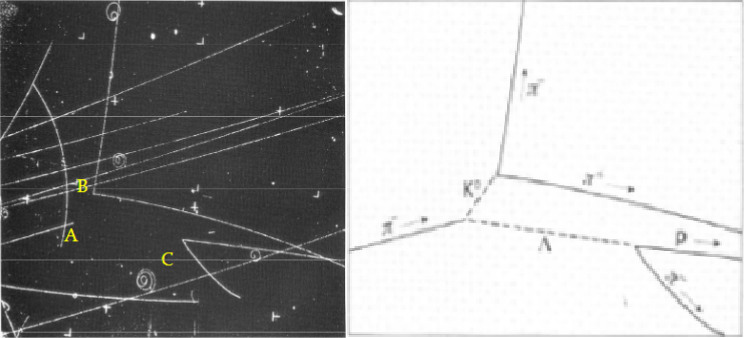
\includegraphics[width=0.7\textwidth]{immagini/fig_bubb_chamb_strange.png}
    \caption{La reazione $A)$ è $\pi^-+p\to K^0+\Lambda$, cioè decade in due particelle neutre che non vediamo; la reazione $B)$ è $K^0\to\pi^-+\pi^+$; la reazione $C)$ è $\Lambda\to p+\pi^-$. A destra vediamo lo schema di ciò che è avvenuto.}
    %\label{}
\end{figure}
\begin{itemize}
\item Dal raggio di curvatura ottengo l'impulso delle particelle cariche e conoscendo la loro massa posso calcolare l'energia.
\item Dalla massa invariante posso ricavare la massa della particella madre:
\begin{equation*}
m_K=\sqrt{\qty(E_1+E_2)^2-\qty(\vec p_1+\vec p_2)^2}
\end{equation*}
\item Dalla massa e dall'energia totale $E_1+E_2$ posso ricavare $\gamma$ e $\beta$. 
\item Dunque misurando il libero cammino medio $\lambda$ (la traccia) ritroviamo il tempo di vita medio
\begin{equation*}
\lambda=\gamma\beta c\tau
\end{equation*}
\end{itemize}
\subsubsection{Perché sono strane?}
\begin{itemize}
    \item La sezione d'urto è dell'ordine del mb, tipico delle interazioni forti. Tuttavia, la vite medie sono dell'ordine di $10^{-10}$ s, tipico dei decadimenti deboli.
    \item Ci sono dei dubbi:
    \begin{enumerate}
        \item Perché $\Lambda\to p+\pi^-$ non avviene tramite interazione forte?
        \item Perché le particelle strane sono sempre prodotte in coppia?
        \item Questa particella carica decade in due modi diversi, stessa massa e vita media ma hanno parità opposta.
    \end{enumerate}
    \item Una spiegazione dell'anomalia fu fornita da Gell-Mann e Pais nel 1954 indipendentemente da Nishijima. Introdussero un nuovo numero quantico, la stranezza, che viene conservata nelle interazioni forti e violata nelle interazioni deboli.
    \item È una simmetria discreta quindi è un numero quantico additivo. Gli adroni già noti, nucleoni e pioni hanno stranezza nulla. Gli iperoni hanno stranezza $-1$ e i mesoni $K$ hanno stranezza $\pm1$. 
    \item Inoltre le particelle strane devono essere prodotte in coppia (produzione associata) con stranezza opposta affinché si conservi.
\end{itemize}
\subsubsection{Produzione di particelle strane}
\begin{itemize}
    \item Vennero utilizzati fasci di $K$ carichi per produrre nuove particelle strane. 
    \begin{gather*}
        K^-+p\to\Lambda+\pi^0\text{ Interazione forte: s si conserva}\\
        \Lambda\to p+\pi^-\text{ Interazione debole: s non si conserva}
    \end{gather*}
    \item A parità di energia, i $K^-$ producono più particelle
    dei $K^+$ perché si producono anche gli iperoni che hanno stranezza -1.
    \begin{figure}[H]
        \centering
        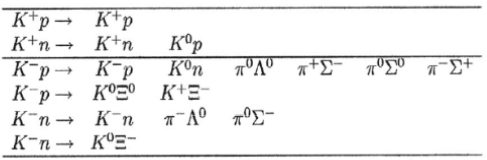
\includegraphics[width=0.6\textwidth]{immagini/fig_strange_prod.png}
        \caption{}
        %\label{}
      \end{figure}
    \item Da raggi cosmici e acceleratori furono trovati sei iperoni strani metastabili.
    \begin{figure}[H]
        \centering
        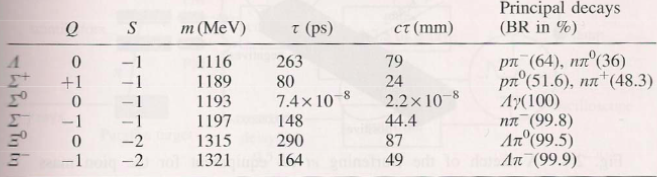
\includegraphics[width=0.6\textwidth]{immagini/fig_iperoni_strani.png}
        %\caption{}
        %\label{}
    \end{figure}
    notiamo che $\Sigma^0$ decade elettromagneticamente, legata a livello energetico che si diseccita ?????? Perché $\Lambda$ ha quei BR?
\end{itemize}
\subsection{Particelle 1}
\subsubsection{Classificazione delle particelle}
\begin{itemize}
\item Nel 1950, nuove particelle e risonanze furono scoperte. Questo fu dovuto al fatto che si iniziarono ad avere a disposizione gli acceleratori e si smise di basarsi unicamente sui raggi cosmici. 
\item Fu fatto un tentativo di classificare tutte queste particelle in modo da rivelarne la vera natura, simile alla tavola periodica. 
\item Una prima simmetria era associata all'isospin; particelle con stesso isospin sono identiche davanti alla forza forte, mentre la forza elettromagnetica (e debole )rompe la simmetria causando una differenza in massa di qualche \% tra le particelle dello stesso multipletto.
\end{itemize}
\subsubsection{Gli adroni sono particelle elementari?}
\begin{itemize}
    \item Col tempo la nozione di particella \textit{elementare} entrò in crisi. L'esistenza di troppi adroni fu vista come una contraddizione rispetto alla natura elementare della componente fondamentale della materia.
    \item Era naturale interpretare gli adroni come risonanze di componenti elementari. Il problema principale divenne quindi misurare le proprietà di queste componenti ed eventualmente osservarle.
    \item Troppi stati adronici, sono allora risonanze? La \autoref{fig:discovery} mostra le scoperte delle particelle dal 1898 agli anni '60; la loro abbondanza e regolarità, in funzione di numeri quantici come carica e stranezza, suggerivano una possibile sequenza, simile alla tavola di Mendeleev.
    \begin{figure}[H]
        \centering
        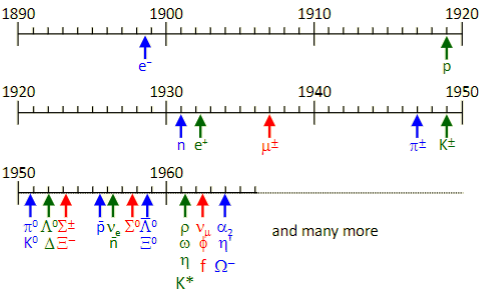
\includegraphics[width=0.7\textwidth]{immagini/fig_discovery.png}
        %\caption{}
        \label{fig:discovery}
    \end{figure}
    \item Per estendere la simmetria, si è tentato di raggruppare diversi multipletti di isospin in un gruppo più grande con lo stesso spin e parità, ma con diversa stranezza (o ipercarica).
    \item Esistono altre possibili scelte a priori, come mantenere la stessa stranezza ma con spin e parità diversi, ma queste opzioni non funzionano.
    \item Nel 1949 Fermi e Yang proposero una strategia per classificare tutte le particelle. Tutte sono descritte da stati legati di protone e neutrone, ed in particolare sono risonanze di questo sistema. Con la scoperta delle particelle strane questo fu scartato (fino a risonanze $\Delta$ funzionava).
    \item Nel 1956 Sakata estese questo modello includendo il $\Lambda$ per tenere conto della stranezza: tutti gli stati adronici erano composti da protone, neutrone e $\Lambda$ e rispettive antiparticelle.
    \item Nel 1961 Gell-Mann e Ne'eman proposero una classificazione delle particelle basata sulla simmetria matematica $SU(3)$, detta \textit{Eightfold Way} (via dell'ottetto). La classificazione non menziona esplicitamente la presenza di una struttura interna. Il nome fu inventato da Gell-Mann e viene dagli otto comadamenti del buddismo.
\end{itemize}
\subsubsection{Simmetrie e gruppi}
Consideriamo ad esempio il gruppo di rotazione.
\begin{itemize}
    \item Due rotazioni successive $R_1$ seguita da $R_2$ sono equivalenti ad una singola rotazione $R=R_2R_1$. Il gruppo in questo caso è \textit{chiuso} rispetto alla moltiplicazione.
    \item Esiste l'elemento identità (no rotazione) e ogni rotazione ha una inversa $R^{-1}$.
    \item Il prodotto non è necessariamente commutativo $R_1R_2\neq R_2R_1$ (dunque non è abeliano), ma vale sempre la proprietà associativa $(R_1R_2)R_3=R_1(R_2R_3)$. Invece nelle rotazioni nel piano vale la proprietà commutativa.
    \item Il gruppo è \textit{continuo}: ogni rotazione può essere descritta da un insieme di parametri che variano continuamente $(\alpha_1,\alpha_2,\alpha_3)$, i quali possono essere considerati come le componenti di un vettore $\vec \alpha$ diretto lungo l'asse di rotazione, con una intensità data dall'angolo di rotazione.
    \item Il gruppo delle rotazioni è un gruppo di Lie: ogni rotazione può essere espressa come il prodotto di una successione di rotazioni infinitesime (arbitrariamente vicine all'identità). Il gruppo è quindi completamente definito dalla “vicinanza all'identità”.
    \item Le rotazioni sono un sottoinsieme delle trasformazioni di Lorentz e formano un gruppo di simmetria di un sistema fisico: la fisica è invariante rispetto alle rotazioni. Infatti consideriamo
    \begin{equation*}
        \ket{\psi}\overset{R}{\longrightarrow}\ket{\psi'}=U\ket{\psi}
    \end{equation*}
    e poiché la probabilità deve restare la stessa:
    \begin{equation*}
        \abs{\braket{\phi}{\psi}}^2=\abs{\braket{\phi'}{\psi'}}^2=\abs{\mel{\varphi}{U^\dag U}{\psi}}^2\implies U^\dag U=1
    \end{equation*}
    cioè $U$ deve essere unitario. Gli operatori $U(R)$ formano un gruppo, in particolare una \textit{rappresentazione unitaria} del gruppo delle rotazioni.
    \item Poiché la hamiltoniana è invariante per operazioni di simmetria $R$ del sistema, gli elementi di matrice si conservano:
    \begin{equation*}
        \mel{\phi'}{H}{\psi'}=\mel{\phi}{U^\dag H U}{\psi}=\mel{\phi}{H}{\psi}\implies U^\dag H U=H\implies\comm{U}{H}=0
    \end{equation*}
    \item La trasformazione $U$ non ha dipendenza esplicita dal tempo e l'equazione del moto 
    \begin{equation*}
        i\dv{\ket{\psi(t)}}{t}=H\ket{\psi(t)}
    \end{equation*}
    è invariante per trasformazioni di simmetria. Dunque il valore di aspettazione di $U$ è una costante del moto.
    \item Tutte le proprietà di gruppo seguono dal considerare rotazioni infinitesime attorno all'identità. Un esempio di rotazione attorno al terzo asse:
    \begin{equation*}
        U=1-i\epsilon J_3
    \end{equation*}
    con $J_3$ generatore delle rotazioni attorno al terzo asse.
    \begin{equation*}
        1=U^\dag U=(1+i\varepsilon J_3^\dag)(1-i\varepsilon J_3)=1+i\varepsilon(J_3^\dag-J_3)+\order{\varepsilon^2}
    \end{equation*}
    dunque $J_3^\dag=J_3$ è hermitiano ed è un osservabile.
    \item Effettuiamo una rotazione $R$ sulla funzione d'onda. Poiché la fisica è invariante per rotazione, abbiamo:
    \begin{gather*}
        \psi'(\vec r)=\psi(R^{-1}\vec r)=U\psi(\vec r)\implies\\ 
        U\psi(x,y,z)=\psi(x+\varepsilon y,y-\varepsilon x,z)=\psi(x,y,z)+\varepsilon\qty(y\pdv{\psi}{x}-x\pdv{\psi}{y})=\psi\qty[1-i\varepsilon\qty(xp_y-yp_x)]
    \end{gather*}
    da cui ne segue che $J_3=xp_y-yp_x$ è il generatore delle rotazioni attorno all'asse $z$, ossia la componente del momento angolare. L'invarianza per rotazioni implica la conservazione del momento angolare.
    \item Per una rotazione finita di $\vartheta$:
    \begin{equation*}
        U(\vartheta)=\qty[U(\varepsilon)]^n=\qty(1-i\frac\vartheta n J_3)^n\to e^{-i\vartheta J_3}
    \end{equation*}
    al solito l'algebra dei generatori è di Lie in quanto vale la relazione
    \begin{equation*}
        \comm{J_i}{J_j}=i\epsilon_{ijk}J_k
    \end{equation*}
    Le funzioni non lineari dei generatori che comutano con tutti i generatori sono dette invarianti o \textit{operatori Casimir}. Per il gruppo di rotazione l'unico operatore Casimir è:
    \begin{equation*}
        J^2=J_1^2+J_2^2+J_3^2\text{ infatti }\comm{J^2}{J_i}=0
    \end{equation*}
    e ne segue che\footnote{Mi ricorda i famosi tre puntini di Marano.} possiamo costruire gli autostati simultanei di $J^2$ e $J_3$:
    \begin{gather*}
        J^2\ket{j,m}=\hbar^2j(j+1)\ket{j,m}\\
        J_3\ket{j,m}=\hbar m\ket{j,m}
    \end{gather*}
\end{itemize}
\subsubsection{Gruppo $SU(2)$}
\begin{itemize}
\item Nella dimensione minore non banale del gruppo delle rotazioni, $j=\frac12$, i generatori sono le matrici di Pauli:
\begin{equation*}
    J_k=\frac12\sigma_k
\end{equation*}
che descrivono particelle con spin $\frac12$.
La matrice di trasformazione è $U(\vartheta_i)=e^{-i\vartheta_i\frac{\sigma_i}2}$. Queste matrici sono unitarie cioè appartengono a $U(2)$. Tuttavia, le matrici di Pauli sono tutte a traccia nulla, dunque in particolare appartengono a $SU(2)$. Si dimostra che ogni matrice hermitiana a traccia nulla $\sigma$ vale:
\begin{equation*}
    \text{det}\,e^{i\sigma}=e^{i\text{Tr}\sigma}=1
\end{equation*}
\item Per un sistema composto valgono le usuali regole del momento angolare. Si ha $J=J_A+J_B$ che soddisfa l'algebra di Lie e gli autovalori $J(J+1)$ ed $M$ di $J^2$ e $J_3$ sono numeri quantici conservati. Dunque abbiamo il prodotto di due rappresentazioni irriducibili $2J_A+1$ e $2J_B+1$ che diventa $2J+1$ nella base $\ket{J_A,J_B,J,M}$, con 
\begin{equation*}
    \abs{J_A-J_B}\leq J\leq J_A+J_B\qquad M=m_A+m_B
\end{equation*}
e per trovare gli autostati su usano i coefficienti di Clebsch-Gordan.
\item Chiaramente è uguale il discorso per l'isospin e le matrici sono le stesse di Pauli. 
\end{itemize}
\subsubsection{slide misteriosa Isospin for antiparticles}
\begin{gather*}
\mqty(p'\\n')=e^{-i\pi \frac{\tau_2}2}=-i\tau_2\mqty(p\\n)=\mqty(0 & -1 \\ 1 & 0)\mqty(p\\n) \\
\mqty(\bar p'\\\bar n')=\mqty(0 & -1 \\ 1 & 0)\mqty(\bar p\\\bar n) 
\end{gather*}
Affinché l'anti doppietto si trasformi come il doppietto, dobbiamo riordinare il doppietto ed introdurre un segno meno:
\begin{equation*}
\mqty(-\bar n'\\\bar p')=\mqty(0 & -1\\1 & 0 )\mqty(\bar p\\\bar n)
\end{equation*}
da cui per nucleone-antinucleone:
\begin{equation*}
    \begin{cases}
        \ket{1,1}=-p\bar n\\
        \ket{1,0}=\sqrt{\frac12}\qty(p\bar p-n\bar n)\\
        \ket{1,-1}=n\bar p
    \end{cases}
\end{equation*}
\begin{equation*}
\ket{0,0}=\sqrt{\frac12}\qty(p\bar p+n\bar n)
\end{equation*}
Non lo so. So solo che 
\begin{equation*}
    \mqty(p\\n)\longrightarrow\mqty(-\bar n\\\bar p)
\end{equation*}
\subsubsection{Gruppo $SU(3)$}
\begin{itemize}
    \item È il gruppo delle matrici unitarie $3\times3$ con determinante unitario. I generatori sono $3^2-1=8$ matrici hermitiane a traccia nulla e linearmente indipendenti. Due di esse sono diagonali. Otto è il numero massimo di generatori che commutano mutualmente (questo vuol dire essere indipendenti), che è dunque il rango del gruppo.
    \item Si può dimostrare che il rango del gruppo è uguale al numero di operatori Casimir.
    \item La rappresentazione fondamentale di $SU(3)$ è un tripletto (e.g. i tre colori di un quark). I generatori sono matrici $3\times3$ indicante con $\lambda_i$, dette \textit{matrici di Gell-Mann}.
    \begin{equation*}
    \lambda_3=\mqty(\dmat{1,-1,0})\qquad \lambda_8=\mqty(\dmat{1,1,-2})
    \end{equation*}
    \item È necessario passare a $SU(3)$ a causa della introduzione di un secondo numero quantico additivo, la stranezza, che assieme ad $I_3$ rende necessario aumentare il gruppo di simmetria. Fu proposto nel 1961. L'assegnazione delle particelle al multipletto $SU(3)$ non è ovvia a causa della elevata differenza in massa tra le varie particelle strane e non strane. 
    \item Ad esempio l'ottetto barionico contiene particelle con differenza di massa fino a 400 MeV, con in media una massa di 1100 MeV.
    \item La simmetria in $SU(3)$ è molto più approssimata rispetto a $SU(2)$ che è solo per l'isospin. Questo è dovuto al fatto che il quark $s$ è molto più pesante di $u$ e $d$. La simmetria $SU(3)$ è alla base del modello a quark ed è utile anche per classificare gli adroni e capire le loro proprietà. 
    \item Invece i colori in $SU(3)$ sono una simmetria esatta.
\end{itemize}
\subsubsection{La via dell'ottetto (1961-1964)}
\begin{itemize}
\item Tutti gli adroni noti negli anni 60 sono classificati nel piano $I_3-Y$.
\item La stranezza, che contribuisce a $Y$, ha l'effetto di allargare la simmetria di isospin dal gruppo $SU(2)$ al gruppo $SU(3)$.
\item Questa simmetria la chiamiamo \textit{flavour} $SU(3)_F$ per distinguerla dalla \textit{color} $SU(3)_C$ che è invece esatta per le interazioni forti in QCD.
\item Le particelle formano multipletti di $SU(3)_F$. Ciascun multipletto contiene particelle che hanno stesso spin e parità intrinseca. La molteplicità base per i mesoni è nove ($3\times\bar3$), che si suddivide in dui multipletti: ottetto + singoletto. Per i barioni invece ci sono ottetti + decupletti.
\item La nascita di $SU(3)$ fu lunga e complicata. Spiegò sia i multipletti di particelle/risonanze note, sia predisse l'esistenza di nuove particelle prima ancora che furono scoperte.
\item Tuttavia, la differenza in massa tra protone e neutrone (o tra i pioni carichi e neutri) è inferiore a qualche MeV, mentre tra pioni e kaoni o protoni e lambda è molto maggiore. Dunque la simmetria di isospin $SU(2)$ è \textit{quasi esatta}, mentre la simmetria di $SU(3)$, che raggruppa particelle strane e non-strane, è sostanzialmente violata.
\item In principio, la scoperta di flavour più pesanti può essere interpretata con gruppi di rango maggiore, ad esempio con $SU(4)$ includiamo il quark charm e così via. Tuttavia, queste simmetrie maggiori sono ancora più rotte, come dimostrato dai valori di massa. Dunque poi non si usano.
\end{itemize}
\subsubsection{Mesoni $J^P=0^-$}
\begin{figure}[H]
    \centering
    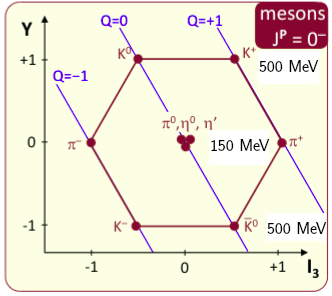
\includegraphics[width=0.5\textwidth]{immagini/fig_mesoni_0_meno.png}
    \caption{Mesoni scalari.}
    %\label{}
  \end{figure}
Nel piano $I_3-Y$ i mesoni $J^P=0^-$ formano un ottetto e un singoletto. Si può osservare come la simmetria di flavour è inesatta dalla differenza in massa ogni scatto di ipercarica. I mesoni $\eta$ sono combinazioni di $u\bar u$, $d\bar d$ e $s\bar s$.
\subsubsection{Mesoni $J^P=1^-$}
\begin{figure}[H]
    \centering
    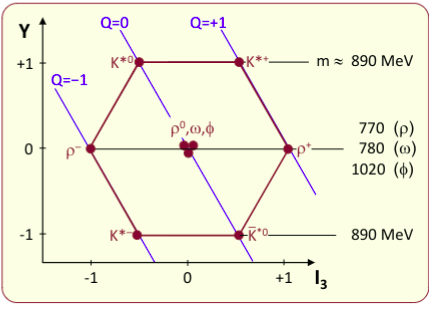
\includegraphics[width=0.5\textwidth]{immagini/fig_mesoni_1_meno.png}
    \caption{Mesoni vettore.}
    %\label{}
  \end{figure}
  Queste sono invece risonanze mesoniche, tutte scoperte nel 1961\footnote{$\phi=s\bar s$, i mesoni $\rho$ sono combinazioni di $u$ e $d$, invece $\omega=\frac1{\sqrt2}(u\bar u+ d\bar d)$}.
\subsubsection{Barioni $J^P=\frac12^+$}
Finora abbiamo considerato solo mesoni dunque $Y=S$. Ora con i barioni avremo $Y=B+S$. 
\begin{figure}[H]
    \centering
    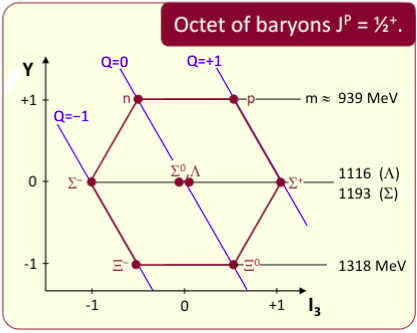
\includegraphics[width=0.5\textwidth]{immagini/fig_baryon_12_piu.png}
    %\caption{}
    %\label{}
\end{figure}
Notiamo come le masse dei mesoni, a causa di $CPT$ che fa passare da kaone ad antikaone, in un ottetto sono simmetriche rispetto $Y=0$ e $I_3=0$, mentre per i baroni la massa aumenta con $S$ perché $m_s>m_u,m_d$. Lo scatto di massa è circa 150 MeV, pattern regolare.
\subsubsection{Barioni $J^P=\frac32^+$}
\begin{figure}[H]
    \centering
    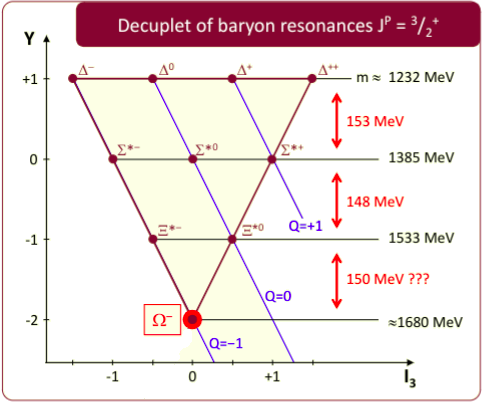
\includegraphics[width=0.5\textwidth]{immagini/fig_baryon_32_piu.png}
    %\caption{}
    %\label{}
\end{figure}
Quando fu proposta la via dell'ottetta, si conoscevano solo nove membri su dieci del decupletto, quindi l'ultimo era una predizione.
\begin{itemize}
\item È un decupletto;
\item La stato $Y=-2,I_3=0(\implies Q=-1, S=-3, B=1)$ deve esistere;
\item Lo si chiama $\Omega^-$;
\item Si guardano le differenze in massa rispetto alla $Y$;
\item Ci aspettiamo che la massa di questa particella sia sui 1680 MeV, che non è una \textit{richiesta obbligatoria} del modello, ma una ragionevole assunzione;
\item Le leggi di conservazione impostano la dinamica della produzione e del decadimento di $\Omega^-$.
\end{itemize}
\subsubsection{La scoperta di $\Omega^-$}
\begin{itemize}
\item Dunque per completare il decupletto manca una particella di stranezza pari a -3.
\item Fu predetta nel 1962 nelle sue varie proprietà: stranezza -3, carica -1, spin $\frac32$, massa 1680 MeV, isospin nullo, ipercarica -2. Fu dunque prevista anche la sua vita media, tipica di quella debole in quando il decadimento forte è proibito, e i principali modi di decadere dovevano essere $\Omega^-\to\Xi^0\pi^-$ oppure $\Omega^-\to\Xi^-\pi^0$ oppure $Omega^-\to Lambda^0K^-$.
\item Può decadere solo in stati con stranezza due. Infatti se decadesse forte (o elettromagneticamente), la reazione più probabile dovrebbe essere $\Omega^-\to\Xi^0K^-$, ma questa è impossibile cinematicamente perché 
\begin{equation*}
m(\Omega)\approx1700\MeV<m(\Xi)+m(K)\approx1800\MeV
\end{equation*}
dunque deve decadere violando la conservazione della stranezza, cioè per interazione debole.
\item Per osservarlo servì sia fortuna che ingegno. Ad esempio la probabilità di conversione di due fotoni in $H_2$ non è elevata. 
\item Dunque si parte da un fascio di $K^-$ in una camera a bolle e si osservano i seguenti decadimenti.
\begin{figure}[H]
    \centering
    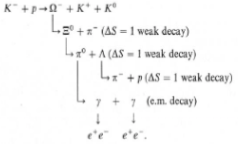
\includegraphics[width=0.55\textwidth]{immagini/fig_omega_meno.png}
    %\caption{}
    %\label{}
  \end{figure}
  Dunque si parte da stranezza -3 e si sempre a diminuire a scatti di 1 decadendo debolmente.
\end{itemize}
\subsection{Il modello statico a quark}
\begin{itemize}
\item Dunque nel 1964 Gell-man e Zweig indipendentemente proposore che tutti gli adroni fossero composti da tre particelle, dette quark (da un romanzo di Joyce).
\item Ancora non era chiaro se questa ipotesi fosse soltanto una convenienza matematica o realtà. Oggi invece sappiamo che i quark sono reali, così come tutte le particelle quantistiche, ma non possono essere osservati come oggetti singoli isolati.
\item Questo modello, che fu poi arricchito con altri altri quark ed interazioni (elettrodebole e QCD), è ancora alla base della nostra comprensione delle particelle elementari: il Modello Standard.
\item Noi considereremo solo le proprietà \textit{statiche} dei tre quark originali.
\item I quark devono essere fermioni in quanto devono essere in grado di formare fermioni e bosoni. In analogia con l'idea di Fermi e Yang, i mesoni sono coppie quark ed antiquark in generale diversi; i barioni (antibarioni) sono stati con tre quark (antiquark).
\item Per formare particelle non strane di carica $0,\pm1$ servono almeno due quarks. Questi devono formare un doppietto di isospin, così che hanno sia $I=0$ che $I=1$.
\item Per formare particelle strane serve un terzo quark, a cui è assegnato per convenzione $s=-1$. \textit{Il numero minimo di costituenti è dunque tre}.
\item Ai quark viene assegnato $B=\frac13$ per sistemare il numero barionico. Inoltre hanno parità $J^P=\frac12^+$.
\item Dalla formula di Gell-Mann e Nishijima ne segue che 
\begin{equation*}
Q(u)=+\frac23\qquad Q(d)=Q(s)=-\frac13
\end{equation*}
dunque i quark hanno carica elettrica frazionaria.
\item I quark formano un tripletto, che è una rappresentazione base del gruppo $SU(3)$. Possono essere rappresentati in forma vettoriale nel piano $I_3-Y$; le loro combinazioni, cioè gli adroni, sono somme di tali vettori.
\begin{figure}[H]
    \centering
    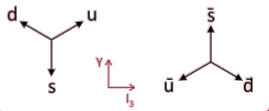
\includegraphics[width=0.4\textwidth]{immagini/fig_quark_vector.png}
    %\caption{}
    %\label{}
  \end{figure}
\end{itemize}
\subsubsection{I mesoni}
\begin{itemize}
    \item Consideriamo per ora solo i quark $u$ e $d$.
    \begin{equation*}
    \mqty(u\\d)\,\mqty(-\bar d\\ \bar u)\implies 
    \begin{cases}
    \ket{1,1}=-u\bar d\\
    \ket{1,0}=\frac1{\sqrt2}\qty(u\bar u-d\bar d)\\
    \ket{1,-1}=\bar ud
    \end{cases}\\
    \ket{0,0}=\frac1{\sqrt2}\qty(u\bar u+d\bar d)
    \end{equation*}
    \item Se aggiungiamo il terzo quark $s$ ci sono 9 possibili combinazioni: un ottetto e un singoletto. Sotto trasformazioni in $SU(3)$ gli otto stati si trasformano tra di loro, ma non si mischiano mai col singoletto.
    \item Dunque costruiamo i mesoni $q\bar q$ con queste regole:
    \begin{enumerate}
    \item Nello spazio $I_3-Y$ sommi i vettori (quark/antiquark) per produrre coppie $q\bar q$, cioè i mesoni.
    \item Tutte le combinazioni sono permesse.
    \end{enumerate}
    \begin{figure}[H]
        \centering
        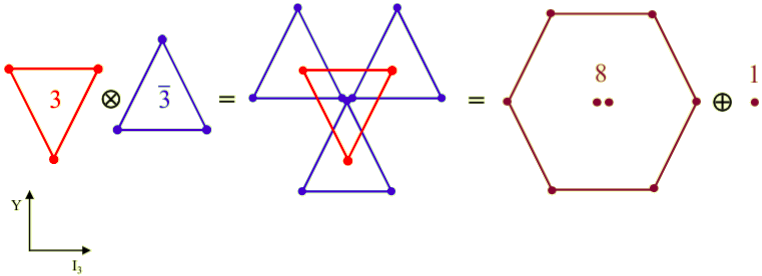
\includegraphics[width=0.6\textwidth]{immagini/fig_mix_meson.png}
        \caption{I mesoni pseudoscalari ($J^P=0^-$) sono gli stati $q\bar q$ in $s$-wave con spin opposti.}
        %\label{}
      \end{figure}
      \item Abbiamo dunque tre mesoni con ipercarica ed isospin nullo. 
\end{itemize}
\subsubsection{Mesoni $J^{PC}=0^{-+}$}
Sono i mesoni in stati di energia più bassa. Specificatamente con $s$-wave otteniamo il nonetto pseudoscalare:
\begin{figure}[H]
    \centering
    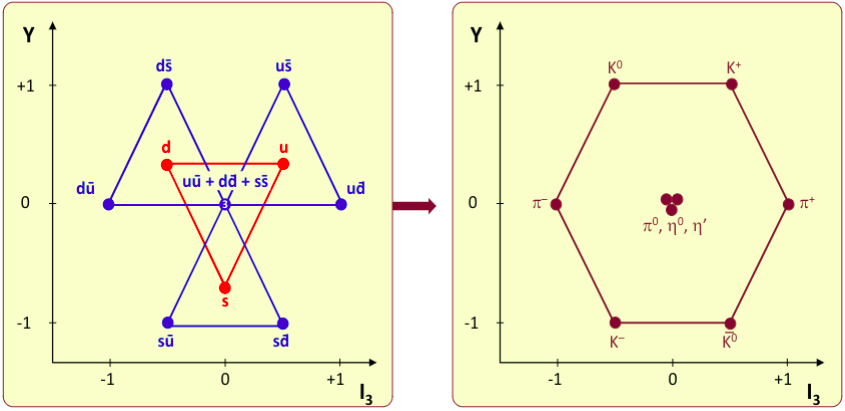
\includegraphics[width=0.7\textwidth]{immagini/fig_pseudoscalar_mesons.png}
    %\caption{}
    %\label{}
  \end{figure}
  Notiamo che $\pi^0,\eta,\eta'$ sono tutte combinazioni (mixing) di tre possibili stati $q\bar q$, come già detto.
  \begin{itemize}
  \item I tre stati con $I_3=Y=0$ sono ortogonali e combinazioni lineari di $u\bar u,d\bar d,s\bar s$.
  \item Indichiamo gli stati con $\{n,\ket{I,I_3}\}$ dove $n$ è la dimensione della rappresentazione (singoletto, doppietto, etc\dots).
  \item Il singoletto di $SU(3)$ deve contenere, per motivi di simmetria, tutti e tre gli stati con stesso peso (una rotazione in $SU(3)$ non cambia lo stato), cioè è puro:
  \begin{equation*}
  \eta_1=\{1,\ket{0,0}\}=\frac1{\sqrt3}\qty(u\bar u+d\bar d+s \bar s)
  \end{equation*}
  \item Ne restano altri due che appartengono all'ottetto. Uno di essi deve appartenere al tripletto con $I=1$, dunque lo possiamo ricavare con gli operatori scala di isospin. 
  \item Così come $p$ ed $n$ formano un doppietto, allo stesso modo $u$ e $d$ e lo stesso per antiparticelle. Poiché $s$ è un singoletto, quando lo aggiungiamo ad un doppietto di isospin non cambia le proprietà del doppietto (cioè considerare $u\bar s$ è come $u$, nel contesto di doppietto).
  \item Le proprietà dell'operatore scala sono le solite:
  \begin{equation*}
  I_\pm\ket{I,I_3}=\sqrt{I(I+1)-I_3(I_3\pm1)\ket{I,I_3\pm}}
  \end{equation*}
  Possiamo vedere varie applicazioni.
  \begin{equation*}
  \begin{cases}
  I_+\ket{d}=\ket{u}\\
  I_+\ket{\bar u}=\ket{-\bar d}\\
  I_+\ket{u}=I_+\ket{\bar d}=0
  \end{cases}
  \begin{cases}
  I_-\ket{1,1}=I_+\ket{1,-1}=\sqrt2\ket{1,0}\\
  I_+\ket{1,0}=\sqrt2\ket{1,1}\\
  I_-\ket{1,0}=\sqrt2\ket{1,-1}\\
  I_+\ket{1,1}=I_-\ket{1,-1}=0
  \end{cases}
  \end{equation*}
  Possiamo applicarlo ad esempio a $\pi^-=-d\bar u$, così da trovare la particella del tripletto $I=1$ con $I_3=0$:
  \begin{equation*}
  I_+\ket{\pi^-}=I_+\ket{-d\bar u}=\ket{-\qty[\qty(I_+d)\bar u+ d\qty(I_+\bar u)]}=\ket{-u\bar u + d\bar d}=\sqrt2\qty(\frac1{\sqrt2}\ket{-u\bar u+d\bar d})=\sqrt2\ket{\pi^0}
  \end{equation*}
  Dunque si definisce
  \begin{equation*}
  \{8,\ket{0,0} \}=\pi^0=\frac1{\sqrt2}\qty(d\bar d-u\bar u)\implies I_+\ket{\pi^0}=\sqrt2\ket{\pi^+}
  \end{equation*}
  \item Resta da trovare l'ultimo. Poiché $s$ ed $\bar s$ sono singoletti, non possono accoppiarsi per dare stati con $I=1$. Possono tuttavia accoppiarsi ad uno stato $I=0$, dunque in generale quest'ultimo stato sarà una combinazione lineare dei tre quark/antiquark. Per trovarlo basta dunque calcolarlo dal generico autostato $a\,u\bar u+ b\, d\bar d + c\,s\bar s$ ed imporre l'ortogonalità con i due già trovati. Risulta
  \begin{equation*}
  \eta_8=\{8,{0,0}\}=\frac1{\sqrt6}\qty(u\bar u+d\bar d-2s\bar s)\qquad I_\pm\eta_8=0
  \end{equation*}
  \item In realtà gli stati fisici sono combinazioni di questi due termini con $s\bar s$, tuttavia siccome l'angolo di mescolamento è piccolo ($\approx11^\circ$), li possiamo identificare in essi stessi.
  \begin{gather*}
  \eta_8:=\eta\qquad m_\eta=548\MeV\\
  \eta_1:=\eta'\qquad m_{\eta'}=958\MeV
  \end{gather*}
  Questo non è totalmente vero, ma c'è poca "contaminazione" come già detto. Infatti uno andrà come il coseno e l'altro come il seno, e l'angolo è piccolo.
  \end{itemize}
\subsubsection{I mesoni $J^{PC}=1^{--}$}
Questi invece sono in un certo senso gli stati eccitati dei precedenti mesoni, infatti il contenuto in quark è spesso lo stesso. In questo caso dunque gli spin sono paralleli.
\begin{figure}[H]
    \centering
    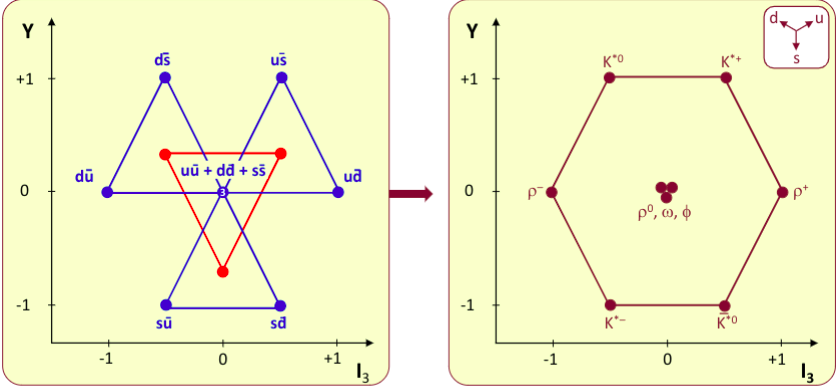
\includegraphics[width=0.7\textwidth]{immagini/fig_vector_mesons.png}
    \caption{Nonetto.}
    %\label{}
\end{figure}
Il contenuto di $K^{0*}$ è lo stesso di $K^0$, e lo stesso per $\rho^-$ con $\pi^-$ e così via. Notiamo che anche $\rho^0$ corrisponde a $\pi^0$, mentre $\omega=\frac1{\sqrt2}(u\bar u+d\bar d)$ e $\phi=s\bar s$ non sono "corrispondenti" a $\eta$ ed $\eta'$.
\subsubsection{Numeri quantici dei mesoni}
\begin{itemize}
    \item Il primo set di mesoni abbiamo detto che hanno $J^{PC}=0^{-+}$, dunque sono $s$-wave cioè hanno $L=0$. 
    \item I quark ed antiquark hanno parità opposta, quindi per i mesoni
    \begin{equation*}
    P(q\bar q)=P(q)P({\bar q})(-1)^L=(-1)(-1)^L=(-1)^{L+1}
    \end{equation*}
    \item Invece riguardo la coniugazione di carica, abbiamo $C=PS$, cioè parità e scambio di spin.
    \begin{figure}[H]
        \centering
        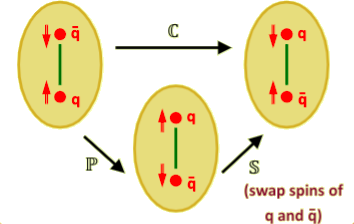
\includegraphics[width=0.6\textwidth]{immagini/fig_charge_conj_mesons.png}
        %\caption{}
        %\label{}
    \end{figure}
    Burcham-Jobes pagina 269: \textit{Ovviamente tante particelle isolate non sono autostati di $C$, ma molti sistemi di particelle possono esserlo se hanno $Q=B=L= S = 0$. Ad esempio un sistema protone-antiprotone system in uno stato di momento angolare definito $l$ (ruotano) e spin $s$ è un autostato di $C$, come adesso mostriamo. Assumiamo che inizialmente l'antiprotone ha coordinate spaziali $x_1$, e si trovi in uno stato di spin $\sigma_1$,mentre il protone è in $x_2$, in uno stato di spin $\sigma_2$. Abbiamo}
    \begin{equation*}
    C\ket{\bar px_1\sigma_1,px_2\sigma_2}=\ket{px_1\sigma_1,\bar px_2\sigma_2}
    \end{equation*}
    \textit{che non è un'equazione agli autovalori ma possiamo renderla tale scambiando spin e posizione. Il protone e l'antriprotone hanno entrambi spin $\frac12$ e quindi possono formare stato di singoletto e tripletto. Il tripletto è simmetrico rispetto allo scambio di spin mentre il singoletto è antisimmetrico. Dunque in scambio di spin appare un fattore $(-1)^{s+1}$. Lo scambio di coordinate è semplicemente una trasformazione di parità che, per il sistema in cosiderazione, dà un fattore $(-1)^l$ dal moto orbitale ed un fattore $(-1)$ dalle parità intrinseche opposte di protone ed antiprotone. Dunque nello scambio abbiamo }
    \begin{equation*}
    C\ket{\bar px_1\sigma_1,px_2\sigma_2}=(-1)^{s+1}(-1)^{l+1}\ket{\bar px_1\sigma_1,px_2\sigma_2}
    \end{equation*}
    \textit{che è una equazione agli autovalori, con autovalori pari a }$(-1)^{l+s}$.
    \item Lo spin intrinseco di un mesone, visto nella sua interezza come particella unica elementare, è $J$ del sistema $q\bar q$.
    \item Ci sono dunque tanti mesoni oltre quelli visti $\pi$ e $\rho$, ed il modo generale per trovarli è con una reazione $p\bar p$ in camera a bolle. Si cercano risonanze (picchi) negli stati finali rispetto a certe masse. Otteniamo una visione molto generale e consistente\dots fu un successo.
    \item Ad esempio possiamo guardare la reazione $\pi^+p\to X$ (con $p_\pi=2.3-2.9\,\GeV$) si hanno le seguenti risonanze:
    \begin{enumerate}
    \item $X=\pi^+\pi^0p$
    \item $X=\pi^+\pi^+\pi^-p$
    \item $X=\pi^+\pi^+\pi^-\pi^0p$
    \end{enumerate}
    La prima è una risonanza $\rho^+(770)\to\pi^+\pi^0$. La seconda è una risonanza $\rho^0(770)\to\pi^+\pi^-$, e la terza è una risonanza $\eta(548)\to\pi^+\pi^-\pi^0$ e $\omega(782)$. Come mai quest'ultimo è una risonanza $\omega$ e non $\rho^0$? Le masse sono simili. È dovuto alla struttura a multipletti di isospin: $\rho^0$ fa parte di un tripletto, $\omega$ è un singoletto. Questo distingue le risonanze.
\end{itemize}
\subsubsection{Decadimento $\rho^0\to\pi^0\pi^0$}
Il decadimento $\rho^0\to\pi^0\pi^0$ è consentito? No, per tre motivi:
\begin{enumerate}
\item \textbf{C-Parity}: abbiamo che 
\begin{gather*}
C(\rho^0)=-1\\
C(\pi^0)=+1
\end{gather*}
dunque, visto che lo stato iniziale è un autostato di $C$, risulterebbe
\begin{equation*}
-1=(+1)\times(+1)\implies \text{NO}
\end{equation*}
La simmetria di $C$ è violata.
\item \textbf{Coefficienti di Clebsch-Gordan nello spazio degli isospin}: 
\begin{gather*}
\ket{\rho^0}=\ket{1,0}\\
\ket{\pi^0}=\ket{1,0}
\end{gather*}
dalla tabella dei coefficienti di Clebsch-Gordan si ha che il sistema $\ket{\pi^0\pi^0}$ ha coefficiente nullo per $\ket{1,0}$ dunque risulta
\begin{equation*}
\braket{\pi^0\pi^0}{\rho^0}=0\implies \text{NO}
\end{equation*}
\item \textbf{Statistica di spin}: sappiamo che $S(\rho^0)=1$ (perché $J=1$), e poiché abbiamo che $S(\pi^0)=0$, per conservare $J$ servirebbe che $L(\pi^0\pi^0)=1$ che è impossibile. Cioè $\rho^0$ è un bosone dunque ha funzione d'onda simmetrica; i due $\pi^0$ sono bosoni identici dunque hanno funzione d'onda spaziale simmetrica; $L=1$ rende la funzione d'onda asimmetrica.
\end{enumerate}
Dunque abbiamo tre motivi per cui non può avvenire $\rho^0\to\pi^0\pi^0$, anche se per dire che è un processo proibito ne bastava una. Una regola generale è: \textit{ un vettore non può decadere in due pseudoscalari uguali.} Tuttavia le prime due \textbf{non} valgono per i decadimenti deboli. Invece la terza ragione è dovuta a statistica e conservazione del momento angolare, che vale per ogni interazione (proibisce anche $Z^0\to HH$, che comunque non può avvenire per motivi di massa).
\subsubsection{Commenti generali sui decadimenti}
\begin{itemize}
\item I decadimenti esistono se nessuna regola di selezione li vieta.
\item Bisogna stare attenti se una regola di selezione è valida per tutte le interazioni o meno, ma soprattutto bisogna stare attenti al fatto che alcune regole \textbf{non} sono ovvie ma sono comunque valide, come $\rho^0\to\pi^0\pi^0$.
\item Le regole di selezione includono:
\begin{enumerate}
\item Numeri quantici come carica, numero barionico, numero leptonico, ecc\dots
\item Conservazione del quadrimpulso, del momento angolare, ecc\dots
\end{enumerate}
\item Per ogni decadimento esiste un elemento di matrice ed una larghezza parziale $\Gamma_i$. Ciascuno di essi contribuisce alla larghezza totale.
\item Per una particella, le $\Gamma_i$ parziali possono variare molto, principalmente a causa dei loro accoppiamenti, e.g. $\Gamma(\rho^0\to\pi^+\pi^-)\gg\Gamma(\rho^0\to e^+e^-)$.
\item Nella pratica quando un decadimento forte esiste, è quello dominante. Gli altri decadimenti hanno probabilità piccole ma non nulle, ad esempio $BR(\rho^0\to e^+e^-)\approx4.7\times10^{-5}$.
\item Inoltre i modi di decadere e le rispettive larghezze $\Gamma$ sono specifiche per ogni processo e non necessariamente simili per particelle simili. e.g. $\Gamma(\pi^\pm)\ll \Gamma(\pi^0)$, oppure il protone è stabile mentre il neutrone ha $\tau_n\sim879$ s.
\end{itemize}
\subsubsection{Mescolamento dei mesoni}
\begin{itemize}
\item I mesoni sono stati legati $q\bar q$. Consideriamo solo i quark $uds$ (e le antiparticelle) nei nonetti ($J^P=0^-,1^-$).
\item Gli stati $\pi^+=u\bar d,\pi^-=d\bar u, K^+=u\bar s, K^-=s\bar u, K^0=d\bar s, \bar K^0=s\bar d$ non hanno ambiguità di quark.
\item Ma $u\bar u, d\bar d, s\bar s$ hanno gli stessi numeri quantici dunque i tre stati $\psi_{8,0},\psi_{8,1},\psi_{1}$ si mescolano come già visto (due angoli per nonetto).
\item Le particelle fisiche sono $\pi^0,\eta,\eta'$ per $0^-$, mentre sono $\rho^0,\omega,\phi$ per $1^-$ e sono tutte combinazioni lineari di $q\bar q$.
\item Gli angoli di mescolamento per pseudoscalari e vettori si calcolano\dots argomento per curriculum NPP. Lo metto tra un po' prima dei barioni. Rompiamo la quarta parete? Ok la ho appena demolita.
\item Le ampiezze di decadimento dei canali elettromagnetici si possono calcolare e confrontare con l'esperimento. Cerchiamo stati finali con coppie elettrone-positrone, prodotti dal $\gamma$.
\item Ci sono alcuni problemi al riguardo:
\begin{enumerate}
\item I valori sono molti piccoli, e.g. $BR(\rho^0\to e^+e^-)\approx4.7\times10^{-5}$. Ovviamente i decadimenti dominanti di $\rho^0,\omega$ e $\phi$ sono forti; tuttavia alcuni decadimenti elettromagnetici, con bassa sezione d'urto, sono rivelabili. Dunque si misurano le larghezze elettromagnetiche e si confrontano le cariche dei quark.
\item Il fattore di fase è importante, soprattutto per $\phi$, che è molto vicino alla soglia $s\bar s$ ($m_\phi-2m_K=$ pochi MeV).
\end{enumerate}
\item Se questi processi sono elettromagnetici, la sezione d'urto (o larghezza) è proporzionale al quadrato della carica della particella coinvolta. Cioè
\begin{equation*}
M\_{fi}(\rho^0\omega\phi\to e^+e^-)\propto \alpha \sum_i Q_q^i
\end{equation*}
dunque le larghezze saranno:
\begin{gather*}
\Gamma(\rho^0\to e^+e^-)\propto \qty[\frac1{\sqrt2}\qty(\frac23-\frac{-1}3)]^2=\frac12\\
\Gamma(\omega\to e^+e^-)\propto \qty[\frac1{\sqrt2}\qty(\frac23+\frac{-1}3)]^2=\frac1{18}\\
\Gamma(\phi\to e^+e^-)\propto \qty[\frac13]^2=\frac19
\end{gather*}
da cui 
\begin{equation*}
\Gamma(\rho):\Gamma(\omega):\Gamma(\phi)=
\begin{cases}
    \begin{aligned}
        9&:1:2 &\text{teorico}\\
        8.8\pm2.6&:1:1.7\pm0.4 &\text{sperimentale}
    \end{aligned}
\end{cases}
\end{equation*}
dato che lo stato finale è uguale, il rapporto dipende solo dallo stato iniziali. La situazione in generale è motlo chiara: la teoria spiega bene i dati!
\end{itemize}
\subsubsection{SLide 47-50 (WIP)}
\subsubsection{OZI rule (Okubo, Zweig, Iizuka)}
\begin{itemize}
\item Per $\phi$ e per $\omega$ si hanno principalmente tre possibili decadimenti:
\begin{equation*}
\phi\to
    \begin{aligned}
        \begin{cases}
            K^+K^-\qquad &49.1\%\\
            K^0_L K^0_S\qquad &34.4\%\\
            \pi^+\pi^-\pi^0\qquad &15.3\%
        \end{cases}
    \end{aligned}
\qquad\qquad
\omega\to
    \begin{aligned}
        \begin{cases}
            \pi^+\pi^-\pi^0\qquad &88.8\%\\
            \pi^0\gamma\qquad &8.5\%\\
            \pi^+\pi^-\qquad &2.2\%
        \end{cases}
    \end{aligned}
\end{equation*} 
\item Tuttavia, se guardiamo la cinematica (o termine di spazio delle fasi) di $\phi$, il decadimento a $3\pi$ è favorito rispetto ai $2K$.
\begin{gather*}
Q_{3\pi}=m_\phi-2m_{\pi^\pm}-m_{\pi^0}\approx600\,\MeV\\
Q_{2K^0}=m_\phi-2m_{K^0}\approx24\,\MeV\\
Q_{2K^+}\approx32\,\MeV
\end{gather*}
\item A cosa è dovuto questo disaccordo? Alla regola di Zweig (swayig). Il diagramma per il decadimento a $3\pi$ è soppresso perché contiene \textit{linee di quark sconnesse}.
\end{itemize}
\begin{figure}[H]
    \centering
    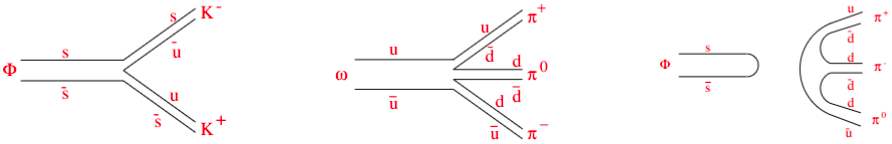
\includegraphics[width=0.8\textwidth]{immagini/fig_ozi_rule.png}
    \caption{Regola di Zweig (OZI).}
    %\label{}
  \end{figure}
\subsubsection{Barioni}
\begin{itemize}
\item I barioni sono semplici da costruire. Basta considerare tre quark. 
\begin{figure}[H]
    \centering
    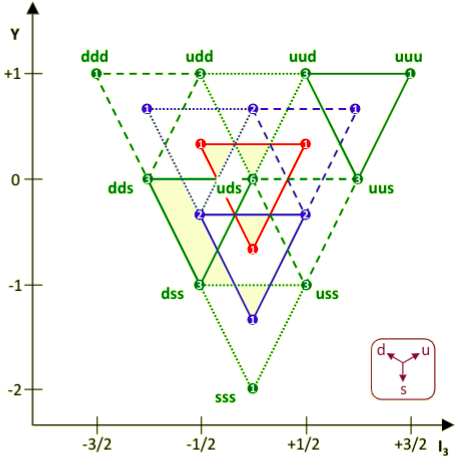
\includegraphics[width=0.5\textwidth]{immagini/fig_baryon_quarks.png}
    \caption{Piano $Y-I_3$ in termini di quark. Ai vertici abbiamo $ddd,uuu,sss$; poi spostandoci nel grafico si scambia un quark con un altro.}
    %\label{}
\end{figure}
\item Quando accoppiamo i tre quark $uds$ otteniamo un decupletto, due ottetti e un singoletto. In realtà il secondo ottetto (e il singoletto) non li vediamo in quanto sono proibiti da conservazione di numeri quantici "che vedremo prossimamente". I tre quark dei barioni hanno sempre $L=0$.
\item "Dimostrazione":
\begin{gather*}
(3\otimes3)\otimes3=(6\oplus\bar3)\otimes3\implies\\
1)\,6\otimes3=10\oplus8\\
2)\,\bar3\otimes3=8\oplus1
\end{gather*}
\end{itemize}
\subsubsection{Barioni: ottetto con $J^P=\frac12^+$}
\begin{itemize}
\item Il multipletto a massa inferiore è un ottetto, che contiene protone e neutrone, un tripletto con $S=-1$ (le $\Sigma$), un singoletto con $S=-1$ (il $\Lambda$), e un doppietto con $S=-2$ (i $\Xi$ detti anche \textit{cascade}).
\begin{figure}[H]
    \centering
    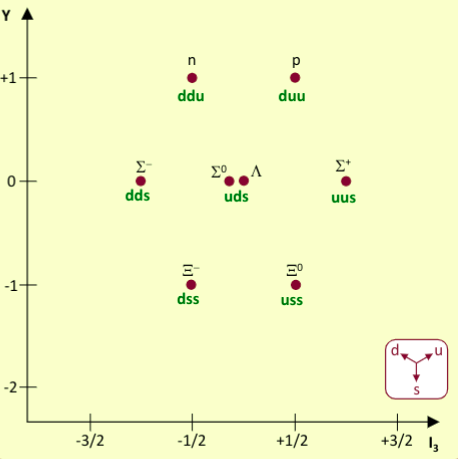
\includegraphics[width=0.5\textwidth]{immagini/fig_baryon_12_quarks.png}
    \caption{I tre quark hanno $l=0$ e spin $\uparrow\uparrow\downarrow$, i.e. spin totale $\frac12$.}
    %\label{}
  \end{figure}
  \item Le masse sono
  \begin{gather*}
  \approx940\,\MeV\text{ per protone e neutrone}\\
  \approx1115\,\MeV\text{ per il }\Lambda\\
  \approx1190\,\MeV\text{ per le }\Sigma\\
  \approx1320\,\MeV\text{ per le }\Xi
  \end{gather*}
  \item La differenza è inferiore a qualche MeV in ciascun multipletto di isospin, a causa della interazione elettromagnetica. 
\end{itemize}
\subsubsection{Barioni: decupletto con $J^P=\frac32^+$}
